\section{Introduction}
\emph{Project Management} functionality is accessible to the \emph{manager} and \emph{administrator} roles
only. Managers can access and modify content created by themselves only, while administrators can see and edit all content available in the system.

From the home page you
can either use available shortcuts, or you can access even more options from the
\emph{Projects} menu on the top. As a manager you will see options as shown in
Figure~\ref{fig:manager-home-page}, while as an administrator you will see more options (see Figure~\ref{fig:admin-home-page}).

\begin{figure}[htb]
\centering
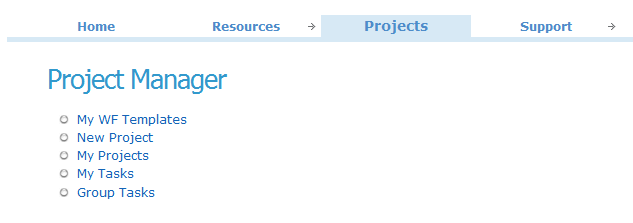
\includegraphics[scale=0.5]{manager-home-page}
\caption{Project menu for \emph{managers}}
\label{fig:manager-home-page}
\end{figure}

\begin{figure}[htb]
\centering
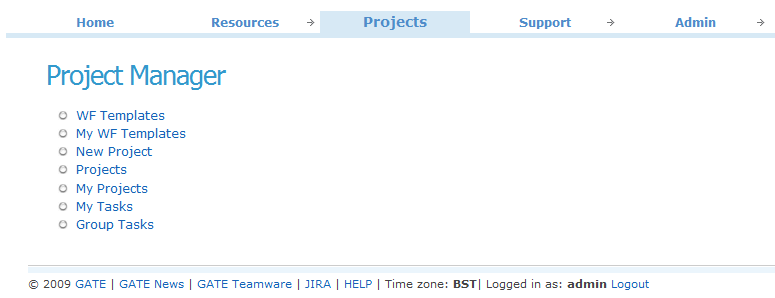
\includegraphics[scale=0.5]{admin-home-page}
\caption{Project menu for \emph{administrators}}
\label{fig:admin-home-page}
\end{figure}


\emph{Annotation projects} are meant to support the following annotation
modules: 

 \begin{itemize}
   \item \emph{automatic}
   \item \emph{manual}
   \item \emph{post-manual (consensus)}
   \item \emph{review}
   \item \emph{post-processing (final consensus)}
 \end{itemize}

You can use any particular module or all of them in the predefined order.
If you want use \emph{manual} or \emph{review} module, you will be able to manage
annotators and curators and specify annotation rules. 

In case of \emph{automatic}, \emph{post-manual}  or \emph{post-processing} 
mode you can choose from existing GATE services (GAS) which can be executed in
sequence. Please see the \emph{Annotation Services} chapter for more details. 

The motivation for combining all modules is to use pre-processing to
bootstrap the manual annotation process. The result of
manual annotation result is consolidated by using post-manual module, in other
words the annotation sets created by human annotators, e.g. \emph{annotator1/2}
are inspected and merged. The identical annotations are moved to \emph{consensus} annotation set and the
different ones are left in \emph{annotator1/2}.
Review process should validate the annotations in \emph{annotator1/2} and
delete false ones. This will leave only reviewed annotations in
\emph{annotator1/2}.

Finally, the remaining - valid annotations in \emph{annotator1/2} are copied to
\emph{consensus} set by post-processing module.

\section{Create new WF template}\label{section:create-new-template}
To create new project, it is mandatory to create Workflow (WF) template first.
Templates are later accessible for creating similar projects.

To create new template, you need to choose \emph{Projects $>>$
My WF Templates $>>$ Create New WF Template with Wizard} option from the top
menu. The wizard will then
guide you through the process of creating template as explained next in Section
~\ref{section:workflow-template-wizard}.

Another way to create new template is during the creation of New project (
explained later in Section
~\ref{section:create-new-project}) by selecting option
\emph{Blank template} at the list of available templates. Click \emph{Select}
button, and you will be redirected to the \emph {Workflow Template} page, from
where you are entering \emph {Workflow Template Wizard}.

\subsection{Workflow Template Wizard}
\label{section:workflow-template-wizard}
\begin{figure}[hb!]
\centering
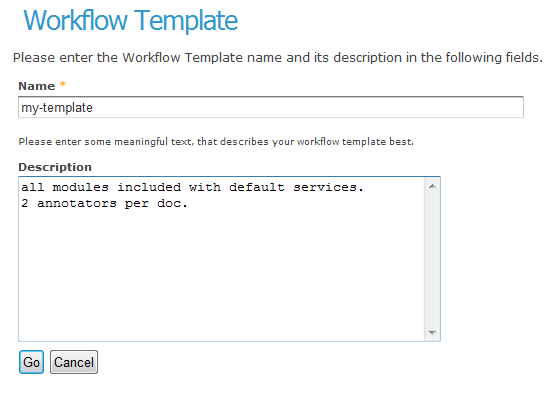
\includegraphics[scale=0.4]{createwftemplate}
\caption{Create New Workflow template}
\label{fig:createwftemplate}
\end{figure}
You need to provide the \emph{name} and \emph{description} of the template.
These two fields will be later used to show overview of the templates and therefore should
contain useful information to help you distinguish between various templates.
Click \emph{Go} button as shown in Figure~\ref{fig:createwftemplate}).

The wizard comprises several steps, the number of which is not fixed as
each of them depends on the preselected options in the previous step.

\begin{figure}[htb]
\centering
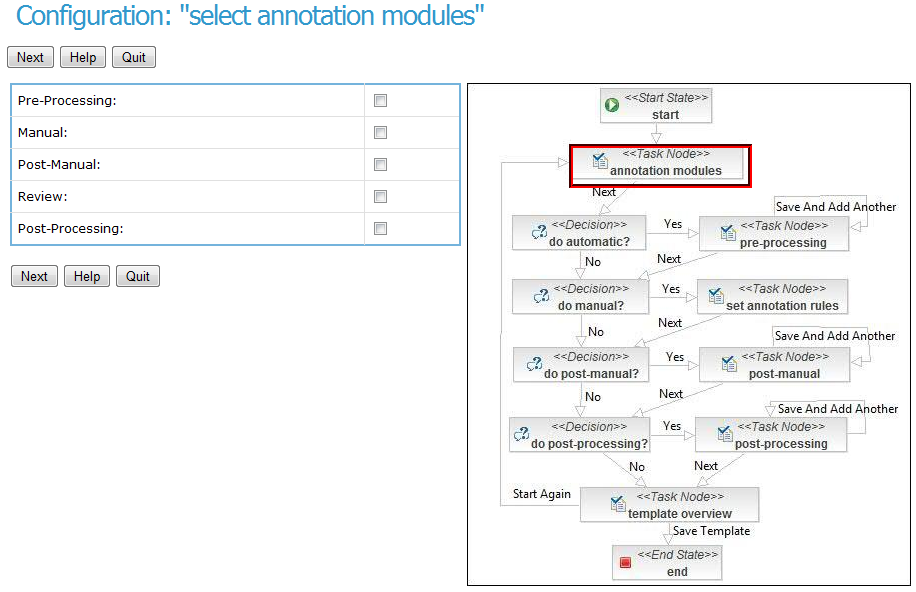
\includegraphics[scale=0.4]{selectannotationmodes}
\caption{Configuration: Select Annotation Modules}
\label{fig:selectannotationmodes}
\end{figure}

During the wizard, the \emph{progress diagram} on the right hand side will
show your progress by highlighting your current step.

The first step is the \emph{Configuration: "select annotation modules"} step,
where you need to choose one or more annotation modules: \emph{automatic},
\emph{manual}, \emph{post-manual}, \emph{review} and/or
\emph{post-processing}, as shown in Figure~\ref{fig:selectannotationmodes}).

Click \emph{Next}. Depending on the chosen modules, the steps to follow
will vary. Here is the detailed explanation of each possible step in case when
all available modules are selected.
\begin{description}
   \item [Pre-processing:] To configure \emph{pre-processing} you need to select
   one or more pre-processing services. When you are done with selection press 
   \emph{Next}. Alternatively you can add as many services as you want to 
   the pipeline by clicking on the button \emph{Save and add another}. This step
  is shown in Figure~\ref{fig:gaspreprocessing}). 
\begin{figure}[hb!]
\centering
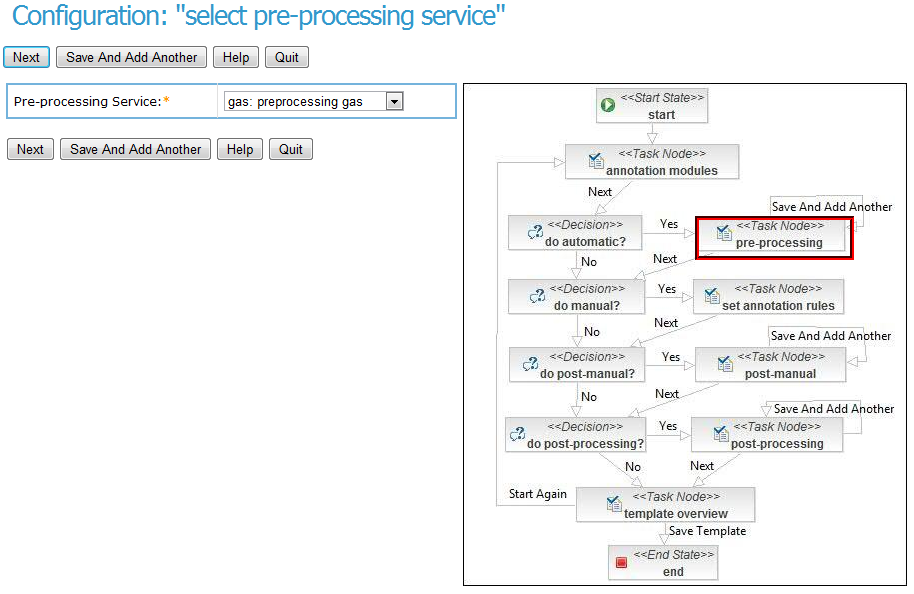
\includegraphics[scale=0.4]{gaspreprocessing}
\caption{Configuration: GAS Pre-processing}
\label{fig:gaspreprocessing}
\end{figure}
    \item  [Manual annotation:] Manual annotation needs a few parameters to be
    specified. This is done in the \emph{Configuration step: "select annotation rules"} 
    as shown inFigure~\ref{fig:selectannotationrules}. Here you will need to:
   \begin{itemize}
       \item select number of annotators per document. For example if you select
       2, each document should be annotated by 2 different annotators;
       \item leave \emph{cancel task allowed} checked; this will allow
       annotators to cancel tasks if they feel unsure about how to annotate the
       document correctly;
       \item leave \emph{anonymous annotation} checked; this will create
       generic annotation set names for annotators (e.g., \emph{annotator1},
       annotator2, etc.) instead of using their usernames. This option is
       useful when you later search annotation sets within documents in
       generalised fashion (for example, using regular expression 'annotator*');
       \item select some of the existing annotation schemas which will be
       loaded inside the Annotation Editor during the process of manual
       annotation (you also have the option to add new schema, if you want).
       \item choose the service which will prepare manual annotation task 
       (copy preprocessed annotations into annotator's annotation set)
   \end{itemize}
 \item  [Post-Manual: and Post-Processing] In \emph{Configuration steps:
   "select post-manual service"}, you can select one or more
   post-manual/post-processing services as shown in
   Figure~\ref{fig:selectpostmanual}. These steps are identical to
   \emph{pre-processing}. The main point is that you can chain services in the order you like 
   and make them executed in a pipeline.
\begin{figure}
\centering
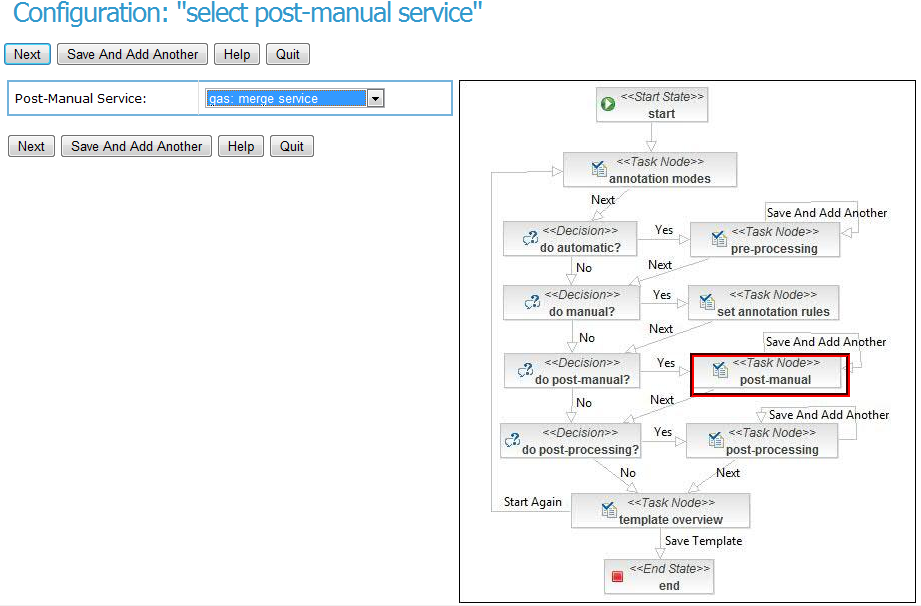
\includegraphics[scale=0.38]{selectpostmanual}
\caption{Configuration: Select Post-Manual}
\label{fig:selectpostmanual}
\end{figure}
\end{description}


From the \emph{Configuration: "template overview"} page
(Figure~\ref{fig:templateoverview}) the template can be saved by clicking on the
\emph{Save template} button. You will be redirected to the
 \emph{My WF Templates} page. Note that if you are not happy with the settings,
 you can repeat the setup procedure by pressing \emph{Start Again} button.
\begin{figure}
\centering
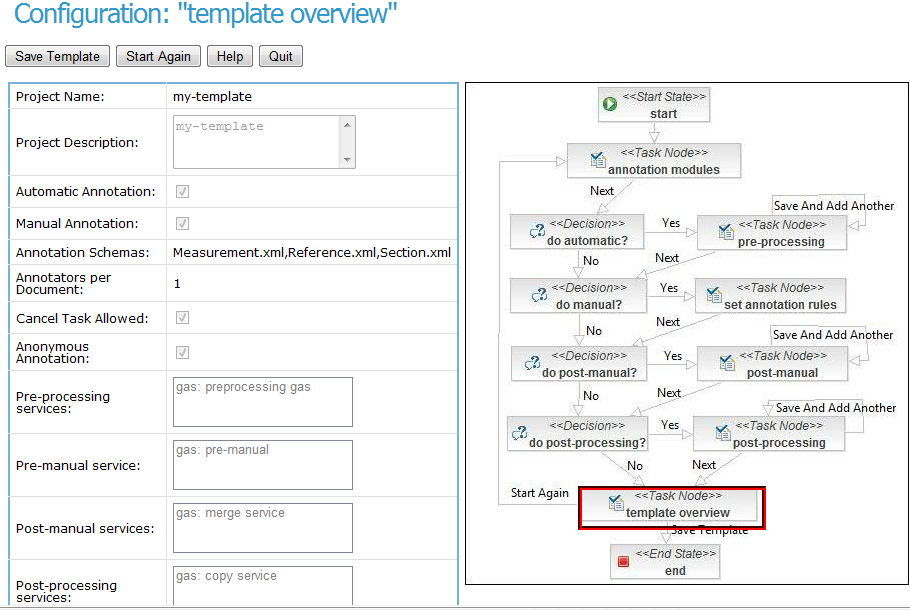
\includegraphics[scale=0.38]{templateoverview}
\caption{Configuration: Template Overview page}
\label{fig:templateoverview}
\end{figure}

At any time you can get more information on the current step or instructions
on how to proceed by hovering over the
 \emph{Help} button. This is especially useful in cases when you are not
sure on how to complete the step.
Quitting the wizard is always possible by pressing the \emph{Quit}
 button. After the warning, and choosing the option \emph{Yes}, the wizard will
 exit, but it can be resumed any time by selecting \emph{Projects $>>$ My WF
 Templates}, and then by clicking \emph{Resume} button for the selected
 template.



\section{My WF templates}\label{section:wf-templates}
Choose \emph{Projects Menu $>>$My Workflow Templates} option from the top menu
or \emph{My Workflow Templates} link at your home page.
You will enter \emph{My WF Templates} page as shown in Figure
~\ref{fig:mywftemplates}.
\begin{figure}[htb]
\centering
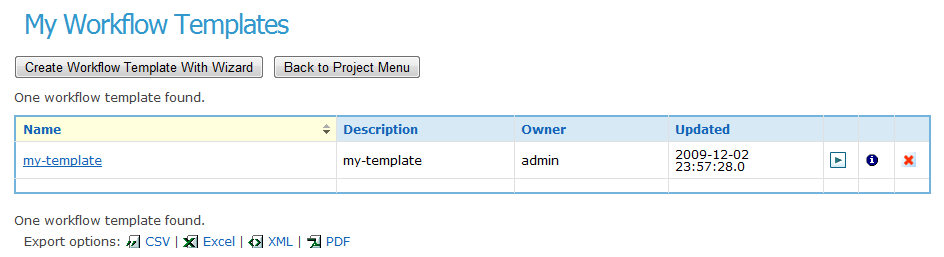
\includegraphics[scale=0.4]{mywftemplates}
\caption{My Workflow Templates}
\label{fig:mywftemplates}
\end{figure}
As we have mentioned previously in Section~\ref{section:create-new-template},
you will land on this page after finishing wizard successfully. In this case,
the status of workflow template will be \emph{Ready}, meaning that you can
create project based on this template (the \emph{Create Project} icon will be
visible only if the template is ready). If during the wizard you quit the
process before finishing template setup, the status of the template will be
\emph{Not Configured}. By clicking on \emph{Resume} icon, you will be able to
resume the setup and complete unfinished steps.

If you want to delete a \emph{Workflow Template}, you can do so by clicking on
the \emph{Delete} icon. Note that all projects based on selected template will
be deleted.

Of course, you will often need to check what configuration is saved in template.
This can be done by hovering \emph{I} icon.

\section{Create new project}\label{section:create-new-project}

For your convenience, there are several ways to create project.
Two have been already mentioned:
 \begin{itemize}
   \item from the corpora list page, you can create project for the specified
corpus by clicking on \emph{Start Project} icon (see
Section~\ref{section:corpora-list}).
   \item from the My Workflow Templates page, you can create project for the
specified template by clicking on \emph{New project} icon (see
Section~\ref{section:wf-templates}).
 \end{itemize}
 
 Here we will cover other ways.
 
From the top menu select "Projects" $>>$ "New Project", or access it 
  directly from the home page. You will be redirected to \emph{Create New 
  Project} page where you need to choose \emph{WF Template}. Here
  you have two options (see Figure~\ref{fig:createnewproject}):
  \begin{itemize}
    \item Choose from the list of available templates and click \emph{Select}.
    \item Create new template, by selecting option \emph{Blank template}.
    If you choose this option, you will need to follow the steps explained
    in Section ~\ref{section:create-new-template}. 
    After you have finished creating the template, you will be redirected to
    the list of WF templates.
  \end{itemize}
\begin{figure}[htb]
\centering
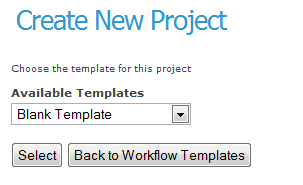
\includegraphics[scale=0.35]{createnewproject}
\caption{Create New Project}
\label{fig:createnewproject}
\end{figure}
You will be redirected to the \emph{Project Data} page where you need to 
provide details of the project. Requested details vary depending on the
annotation modes defined in the WF template. In case you excluded manual
annotation mode, the three options will need to be selected (see
Figure~\ref{fig:projectdata}): project name,
corpus, and manager (you will be selected by default); as a manager of the
project you will be able to see this project in \emph{My projects} list and
manage it (e.g., change actors, monitor project).
\begin{figure}[h!]
\centering
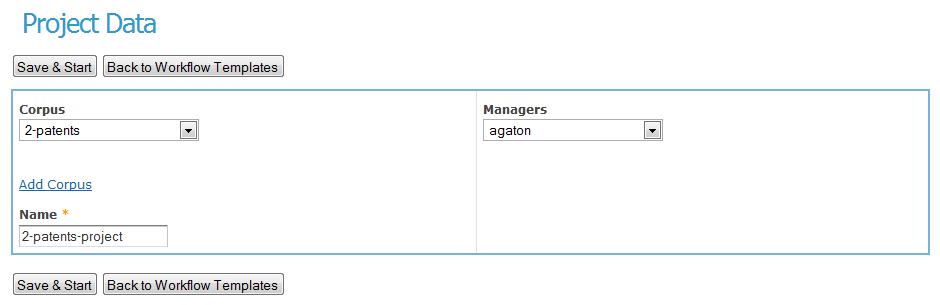
\includegraphics[scale=0.34]{projectdata}
\caption{Configure Project without Manual Annotation}
\label{fig:projectdata}
\end{figure}

When \emph{manual annotation} module is defined, there will be two options in
addition to the previously selected ones: curators and annotators
(see Figure~\ref{fig:projectdatamanual}).
\begin{figure}[htb]
\centering
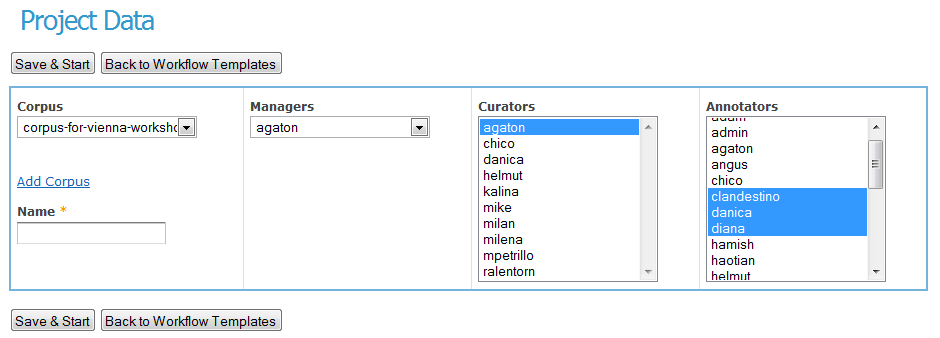
\includegraphics[scale=0.34]{projectdatamanual}
\caption{Configure Project with Manual Annotation}
\label{fig:projectdatamanual}
\end{figure}
For example, you can leave yourself as \emph{manager} and \emph{curator}, and
you can select as many annotators as you wish in the list (hold Ctrl while
selecting annotators for multiple selection of actors).

On the other hand, if you chose \emph{review} module and ommit \emph{manual
annotation} module, there will be an option to select only curators and manager,
since annotators do not take part in review process.

Click \emph{Save \& Start} button and the annotation project will be started.

\section{Annotation Tasks}\label{section:annotation-tasks}

If used template contains manual annotation module all annotators should be
able to get annotation tasks after logging in and clicking on \emph{Open Annotation Editor} from the home page.
We now discuss how annotators (users with \emph{annotator} role execute their
tasks and annotate documents.

As a general rule, users with \emph{Annotator} role assigned, participate in
the project via annotation editor. The annotator's home page contains restricted
operations as shown in Figure~\ref{fig:annotatorhomepage}. The annotator can
either open Annotator editor, or edit his/her profile.
\begin{figure}[htb]
\centering

\includegraphics[scale=0.4]{annotatorhomepage}
\caption{Annotator Home Page}
\label{fig:annotatorhomepage}
\end{figure}

After clicking on \emph{Open annotation editor} link, the annotator has to ask
for the new task. To do this, s/he needs to click on the \emph{Get New Task}
button (the first one from the left side).
Annotation Editor will start to search for available tasks and the annotator
will see the dialogue similar to one shown in
Figure~\ref{fig:getnewtaskineditor}.
\begin{figure}[htb]
\centering
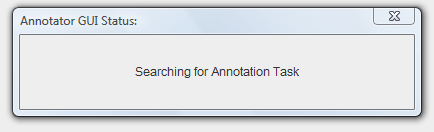
\includegraphics[scale=0.4]{getnewtaskineditor}
\caption{Searching for a new task in Annotation Editor}
\label{fig:getnewtaskineditor}
\end{figure}

If there is an available task, it will be loaded in annotation editor.
The following actions are available (see Figure
~\ref{fig:annotationtaskineditor}):
\begin{itemize}
  \item Finish task (click on the second button from the left) when you finished
with annotations.
  \item Save task (click on the third button from the left) when you want to
save your annotations, but not finish the task.
  \item Reject Task (click on the fourth button from the left) when you feel
unsure how to annotate document and want this to be assigned to other annotator.
\end{itemize}

\begin{figure}[htb]
\centering
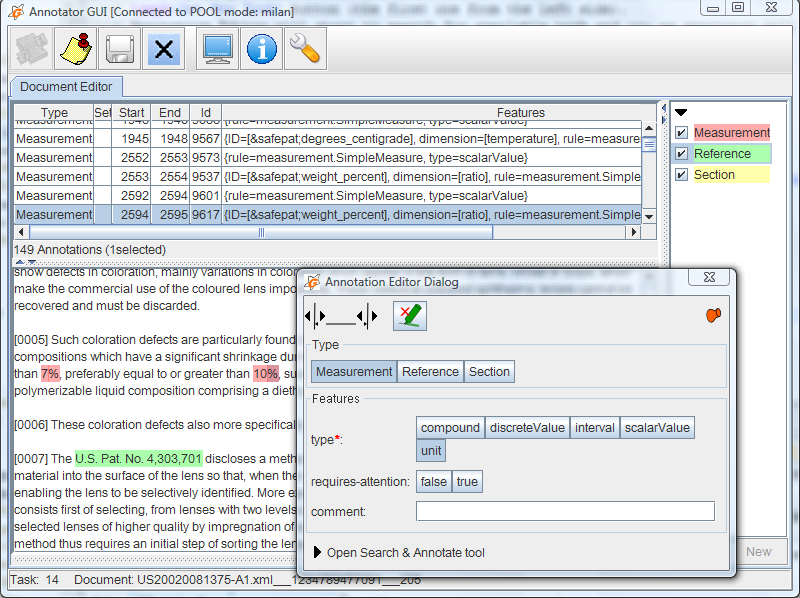
\includegraphics[scale=0.4]{annotationtaskineditor}
\caption{Get New Task in Annotation Editor}
\label{fig:annotationtaskineditor}
\end{figure}

\section{Curation Tasks}\label{section:curation-tasks}
If used template contains \emph{review} module all chosen curators (remember,
you had to select them during project startup) should be able to get curation
tasks after logging in and clicking on \emph{Group Tasks} from the
\emph{Projects Menu} likd shown in Figure~\ref{fig:curator-home-page}. 
\begin{figure}[htb]
\centering
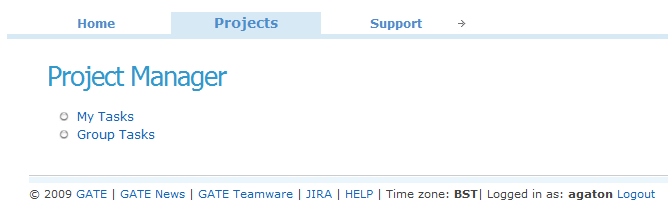
\includegraphics[scale=0.5]{curator-home-page}
\caption{Project menu for curators}
\label{fig:curator-home-page}
\end{figure}

Now we will explain how curator claims and executes his/her tasks and review
documents.

In general, users with \emph{Curator} role assigned, participate in
the project through task form. Since, more than one curator can be assigned to
a particular project, it is necessary for curator to claim his/ger task first,
by clicking on \emph{Accept} icon (see Figure~\ref{fig:reviewgrouptask}). 

\begin{figure}[htb]
\centering
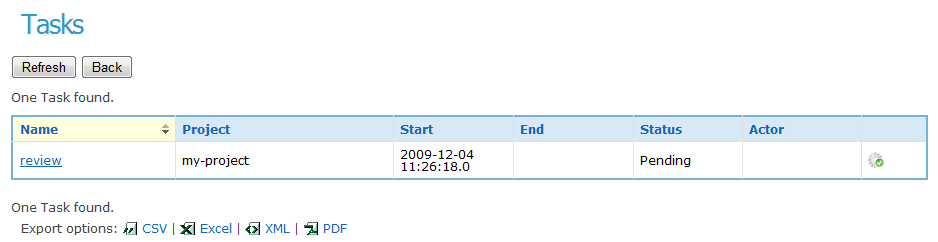
\includegraphics[scale=0.5]{reviewgrouptask}
\caption{Group Tasks}
\label{fig:reviewgrouptask}
\end{figure}

That task will be moved then from \emph{Group Task List} to his/her
\emph{Personal Task list}, as shown in Figure~\ref{fig:acceptedreviewtask} 

\begin{figure}[htb]
\centering
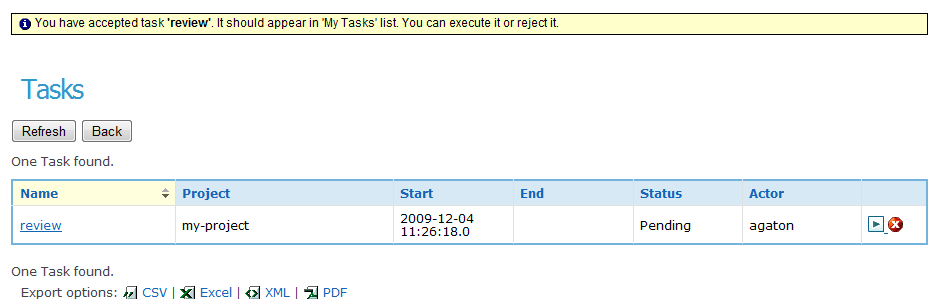
\includegraphics[scale=0.5]{acceptedreviewtask}
\caption{My Tasks}
\label{fig:acceptedreviewtask}
\end{figure}

Curator then executes the task by clicking on \emph{Start} icon.
He will be shown the task form with the instructions which he/she needs to
follow - Figure~\ref{fig:reviewtask} 

\begin{figure}[htb]
\centering
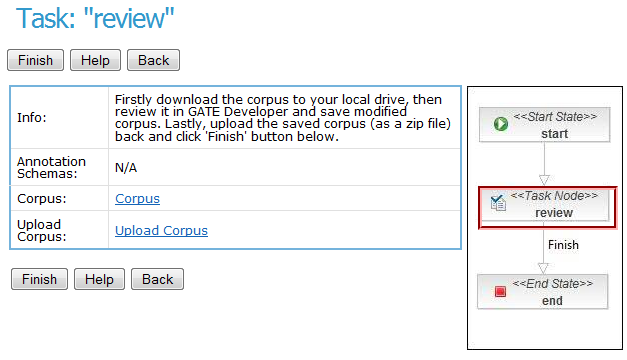
\includegraphics[scale=0.5]{reviewtask}
\caption{Review Task}
\label{fig:reviewtask}
\end{figure}. 

The review procedure briefly comprises the following steps:

\begin{itemize}
  \item Download corpus you need to review as a zip archive, by clicking on
  \emph{Corpus}
  \item Unpack the zip archive and copy documents somewhere on your hard drive
  \item Launch GATE Developer, create new corpus and populate it with the
  unzipped documents.
  \item Run Corpus QA tools (IAA, Annotation Diff, etc) to find out to which
  extent how annotators agree. Note that Corpus QA Tools are added in GATE 5.1.
  \item Delete annotations that you consider false from human annotation sets,
  e.g. \emph{annotator1/2}.
  \item Go back to Teamware, find your task among \emph{My Tasks} and update the
  documents in corpus by clicking on \emph{Upload Corpus} link.
  \item Press \emph{Finish} button in your task form.
\end{itemize}

As a manager you will have more responsibilities than curators and annotators.
One, especially worth mentioning is that managers will be able to manage
projects and have insight into the project progress at any time. In the
following sections we will provide more details on this.

\section{My Projects}
To manage project, select \emph{Projects $>>$ My Projects} from the top menu.
You will see the list of projects that you have created/started, as shown in
Figure~\ref{fig:myprojects}.
\begin{figure}[htb!]
\centering
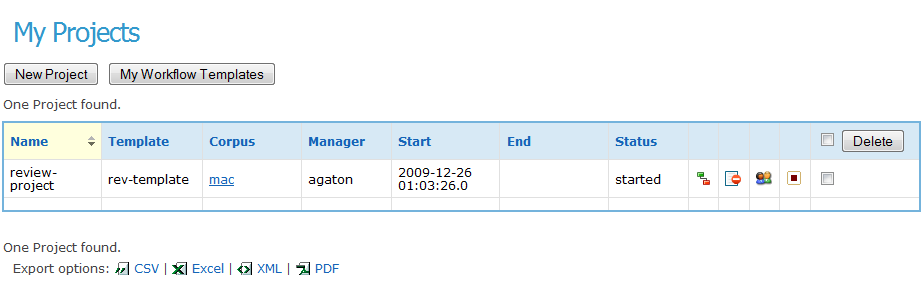
\includegraphics[scale=0.4]{myprojects}
\caption{My Projects}
\label{fig:myprojects}
\end{figure}
For each project, there are several available options (four icons next to the
Status field as shown in Figure~\ref{fig:myprojects}):
\begin{itemize}
  \item \texttt{view processes} for the particular project,
  \item \texttt{suspend/resume} the project,
  \item \texttt{change the project actors}: managers, curators, annotators,
  \item \texttt{end} the project,
  \item \texttt{delete} the project.
\end{itemize}
Besides that, after project is completed, you will be notified by email.
All these options are described in detail in the following subsections.

\subsection{Project Processes}
In order to see project processes, click on \emph{Processes} icon (red and 
green icon, see Figure~\ref{fig:myprojects}) for the specific project listed in
the \emph{My Projects} page.
The process list will be shown as in Figure~\ref{fig:processesinproject}:
\begin{figure}[htb]
\centering
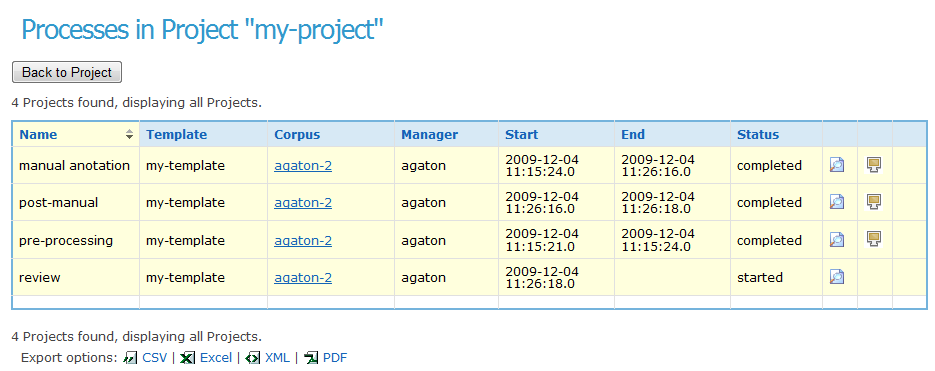
\includegraphics[scale=0.4]{processesinproject}
\caption{Project Processes}
\label{fig:processesinproject}
\end{figure}:
From the \emph{Processes} page, you can:
\begin{itemize}
  \item \texttt{see the status} of each process (started, suspended or
completed),
  \item \texttt{monitor processes} by clicking on \emph{Process Monitoring}
icon. For
details on process monitoring console see details in Section
~\ref{section:process-monitoring}.
  \item \texttt{view tasks} created for each process by clicking on \emph{View
Tasks} icon (see Figure~\ref{fig:taskinstances}).
\begin{figure}[htb]
\centering
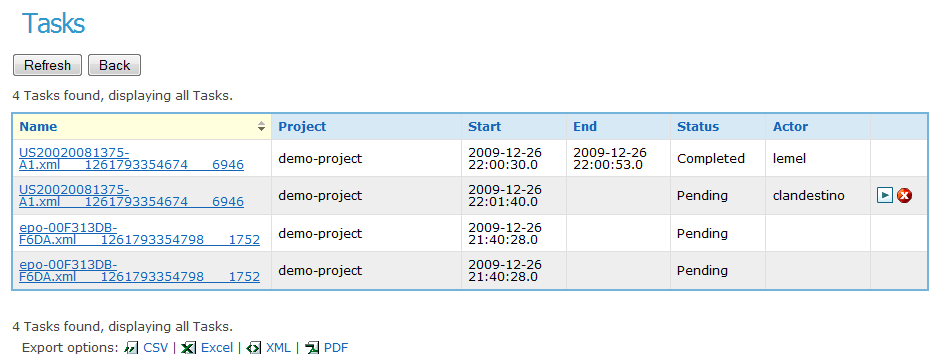
\includegraphics[scale=0.4]{taskinstances}
\caption{Task List}
\label{fig:taskinstances}
\end{figure}
When annotators start to annotate, you will be able to see the list of tasks and
their status. For example, if there are 2
documents in the corpus and 2 annotators are assigned to annotate each document,
there will be 4 tasks in total as shown in Figure~\ref{fig:taskinstances}.
In this example, one annotator finished task, the other annotator accepted the task,
and two left tasks have not been taken yet.
From the Task List page you can also see who is the assigned user, and start and
end times for specific tasks.
Should you want to finish or cancel annotator task, you can do that by
clicking on relevant icons. These actions correspond to \emph{canceling
document annotation} and \emph{returning document to the pool} respectively.
\end{itemize}

\subsection{Suspend/Resume Project}
 A project can be suspended at any time, by clicking on \emph{Suspend} icon.
This means that all processes and tasks in that project will be suspended.
The project can be resumed later, which analogly will result in resuming
its processes and tasks.
This is shown in Figure~\ref{fig:suspendproject}:
\begin{figure}[htb]
\centering
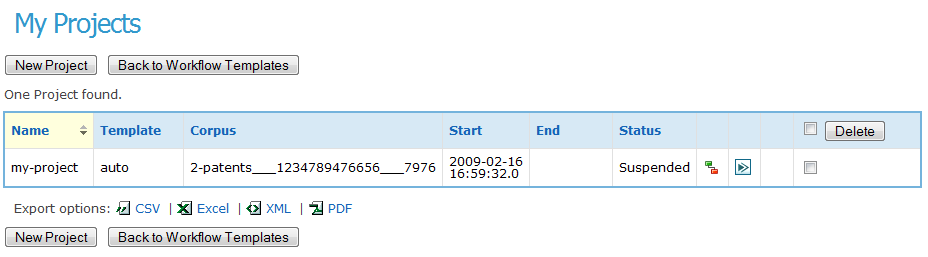
\includegraphics[scale=0.4]{suspendproject}
\caption{Suspend Project}
\label{fig:suspendproject}
\end{figure}

\subsection{Change Project Actors}
There is often a need to change actors during project execution.
For example, you might want to pass manager role to someone else or to change
curators and annotators due to some changes in personnel. This option is
available in GATE Teamware.
From the \emph{My Projects} page you need to click on \emph{Change Actors} icon
for the specific project, and you will be redirected to the page where you can
change all actors as shown in Figure~\ref{fig:changeprojectactors}.
\begin{figure}[htb]
\centering
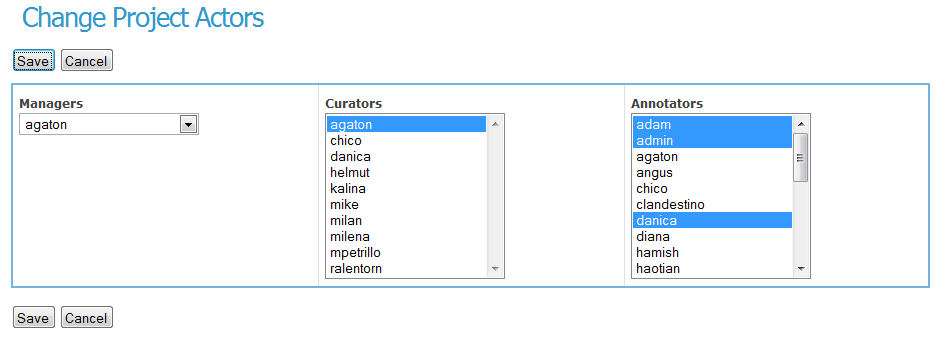
\includegraphics[scale=0.4]{changeprojectactors}
\caption{Change Project Actors}
\label{fig:changeprojectactors}
\end{figure}
As it is visible in Figure~\ref{fig:changeprojectactors}, the current
actors will be preselected.

\subsection{End Project}
 A project can be ended at any time, by clicking on \emph{End} icon (the first
 on the right). This means that all processes and tasks in that project will be
 ended. The project cannot be resumed later. This option is useful if manager wants to 
stop the work on the project, but leave the project history intact.
This is shown in Figure~\ref{fig:endproject}:
\begin{figure}[htb]
\centering
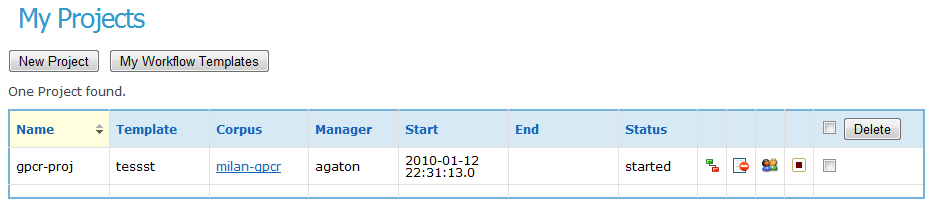
\includegraphics[scale=0.4]{endproject}
\caption{End Project}
\label{fig:endproject}
\end{figure}

\subsection{Delete Project}
With time, the number of your projects will increase, therefore we provide the
option to delete old projects.
It is not restricted only to completed projects, so you can delete even 
running projects. Deleting a project will also delete the
corresponding processes and tasks.

\subsection{Email Notification}
As a manager you will be notified by email, upon your project completion.
This can be very useful, if you are not actively monitoring execution.
The example of email you can expect is shown on
Figure~\ref{fig:projectcompletednotification}.
\begin{figure}[htb]
\centering
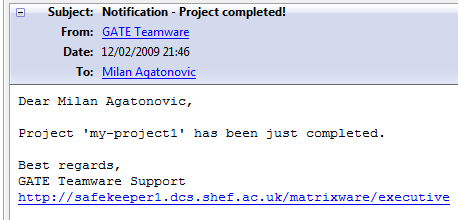
\includegraphics[scale=0.4]{projectcompletednotification}
\caption{Project Completed Notification}
\label{fig:projectcompletednotification}
\end{figure}
\section{Process Monitoring}\label{section:process-monitoring}

Here we will introduce Process monitoring console for real-time
monitoring and gathering information about currently executing processes.
The main idea behind this functionality is to:
\begin{itemize}
  \item isolate annotation process failures,
  \item improve annotation process performance,
  \item help making decisions, and
  \item improve resource management.
\end{itemize}

At the moment, GATE Teamware provides four different views in process
monitoring console:
\begin{itemize}
  \item Document Status Summary
  \item Annotation Status Details
  \item Annotator Record Summary
  \item Record Summary for All Annotators
\end{itemize}

Each view is explained in details in the following subsections.

\subsection{Document Status Summary}
To access this page, click on \emph{Process monitoring} icon in the
process list for particular project. You will see the progress of the
annotation process both in tabular and graphical
view using pie chart as shown in Figure~\ref{fig:annotationstatusoverview}.
\begin{figure}[htb]
\centering
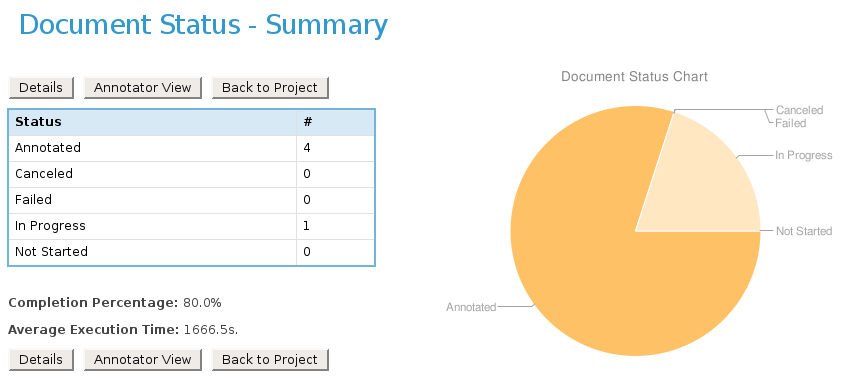
\includegraphics[scale=0.4]{annotationstatusoverview}
\caption{Document Status Summary}
\label{fig:annotationstatusoverview}
\end{figure}
The progress is displayed in real time so that it is possible
 to monitor how many documents have been finished, canceled, annotated, failed,
 in progress, and not started. When the annotation process ends, the pie chart
will disappear.

\subsection{Document Status Details}
Annotation Status Overview gives pretty condensed view about what is going on
inside process.
For more detailed view, click \emph{Details} button, and you will see the
details of the annotation project progress by document, including names of
annotators who started the work on it, finished or
 rejected the document as shown in Figure~\ref{fig:annotationstatusdetailedview}
\begin{figure}[htb]
\centering
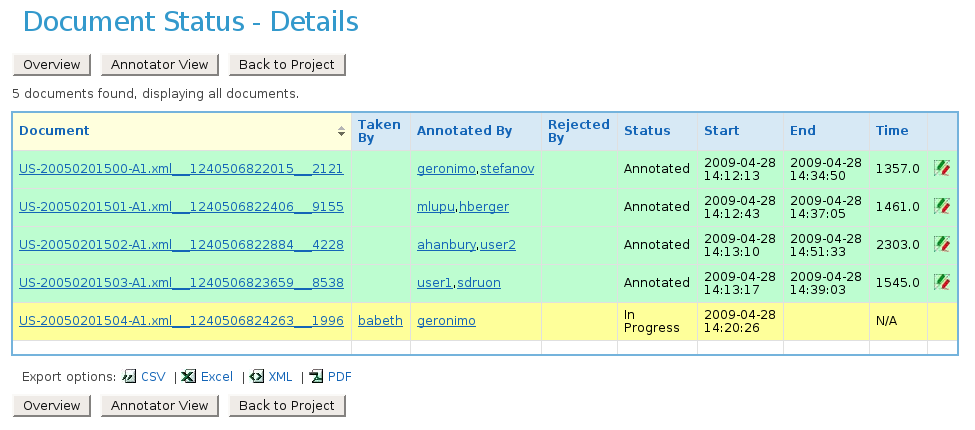
\includegraphics[scale=0.4]{annotationstatusdetailedview}
\caption{Document Status Details}
\label{fig:annotationstatusdetailedview}
\end{figure} 
 
 From this list, the status of the documents is also
 visible together with the execution time per document. For specific documents in
 the list it is possible to view details such as:
 \begin{itemize}
   \item \texttt{view (annotated) documents}, by following the document
name link. This will launch \emph{Annotation Editor}, which is described in
Section ~\ref{section:annotation-editor}
   \item \texttt{compare document annotations}; to do this follow the icon
at the end of the \emph{annotated} document row. The document with
   annotations will be loaded into the \emph{Annotation Differ} application,
which is described in Section ~\ref{section:annotation-differ}
\end{itemize}
 
\subsection{Annotator Record View}
Both annotation status views explained above are focused on the document
itself, while there might be the cases when the manager wants to see how
particular annotator performed. Therefore, we have implemented \emph{Annotator
Record View}, which you can access by clicking on the annotator name from
\emph{Document Status Details} page.
You will be able to see how many documents annotator completed, canceled,
started to annotate, along with some useful metrics. A sample \emph{Annotator
Record View} page is shown in Figure~\ref{fig:annotatorrecordview}:
\begin{figure}[ht!]
\centering
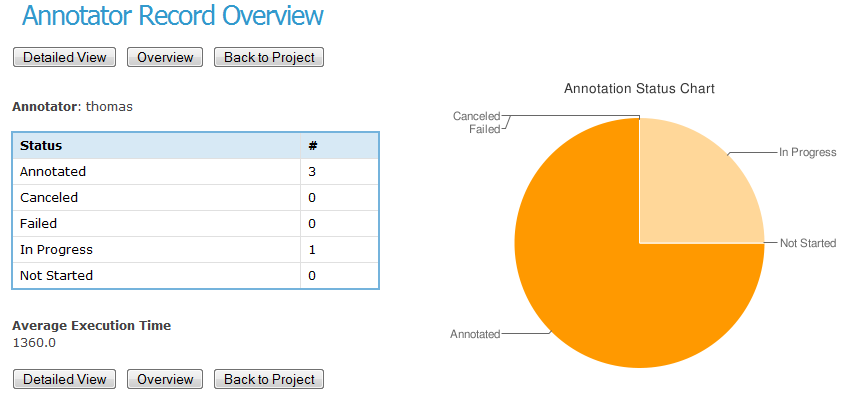
\includegraphics[scale=0.4]{annotatorrecordview}
\caption{Annotator Record View}
\label{fig:annotatorrecordview}
\end{figure}


\subsection{Record Summary for All Annotators}
In case that manager is interested to see how workload is shared among
annotators with an indicator about the average time spent per document,
\emph{Record Summary for All Annotators} screen can be very useful.
You can see this screen by clicking on \emph{Annotator View} button.
An example of this screen is shown in
Figure~\ref{fig:globalannotatorrecordview}: 
\begin{figure}[ht!]
\centering
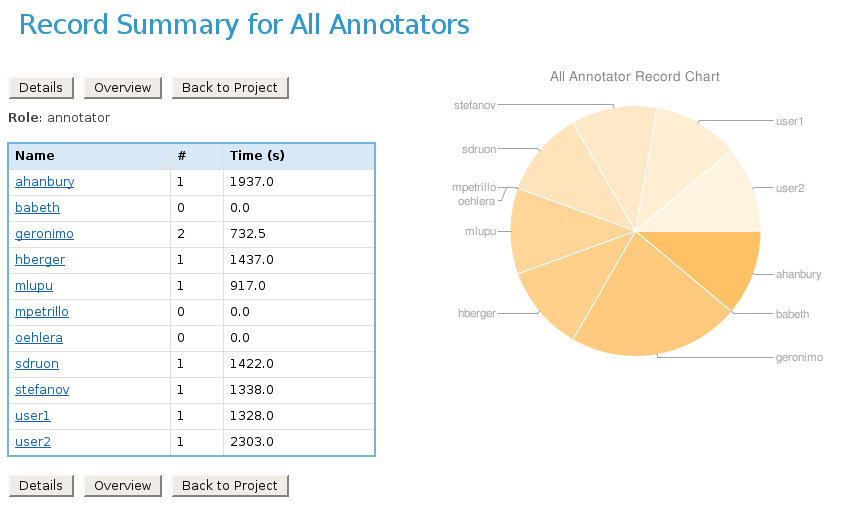
\includegraphics[scale=0.4]{globalannotatorrecordview}
\caption{Global Annotator Record View}
\label{fig:globalannotatorrecordview}
\end{figure}


